\documentclass[french]{article}
\usepackage[T1]{fontenc}
\usepackage[utf8]{inputenc}
\usepackage{amsmath}
\usepackage{fixltx2e}
\usepackage{graphicx}
\usepackage[french]{babel}
\usepackage{color}
\usepackage{colortbl}
\usepackage{listings}
\usepackage{pxfonts}
\usepackage[french]{algorithm2e}
\usepackage{url}
\usepackage{stmaryrd}
\usepackage{wrapfig}
\usepackage{textcomp} % \textlnot
\usepackage{ dsfont } % Z
\usepackage{amssymb}
\usepackage{ textcomp } % times
\usepackage{calc} % strikethrough
\usepackage[normalem]{ulem} % underline
\usepackage{mathrsfs} % \mathscr

% User packages
\usepackage{lstlangarm}

\lstset{
    language=Caml,
    basicstyle=\ttfamily,
    keywordstyle=\color[rgb]{0.5,0,0}\bfseries,
    commentstyle=\color[rgb]{0.133,0.545,0.133},
    showstringspaces=false,
    frame=tb,
    columns=fullflexible,
    morekeywords={undefined}
}

\newtheorem{theorem}{Theorème}

\newcommand\ccc[1]{\color{red}{#1}\color{black}} % TOLDO : check this is unused
\newcommand\SAT{\texttt{SAT}}
\newcommand\UNSAT{\texttt{UNSAT}}
\newcommand\si{\textit{si}}
\newcommand\sinon{\textit{sinon}}

\newcommand*\quotefont{\fontfamily{LinuxLibertineT-LF}} % selects Libertine as the quote font

% define strikethrough
\newsavebox\CBox
\newcommand\strike[2][0.5pt]{%
  \ifmmode\sbox\CBox{$#2$}\else\sbox\CBox{#2}\fi%
  \makebox[0pt][l]{\usebox\CBox}%  
  \rule[0.5\ht\CBox-#1/2]{\wd\CBox}{#1}}

% define bijection map arrow
\def\mathrlap{\mathpalette\mathrlapinternal}
\def\mathrlapinternal#1#2{%
        \rlap{$\mathsurround=0pt#1{#2}$}%
}
\def\bijmap{\ensuremath{%
        \mathrlap{\rightarrowtail}\rightarrow}}

\definecolor{Gray}{gray}{0.85}

\makeatletter
\renewcommand{\@algocf@capt@plain}{above}% formerly {bottom}
\newcommand{\pushline}{\Indp} % Indent
\newcommand{\popline}{\Indm}  % Undent
\newcommand{\pushright}[1]{\ifmeasuring@#1\else\omit\hfill$\displaystyle#1$\fi\ignorespaces} % push to right
\newcommand{\pushleft}[1]{\ifmeasuring@#1\else\omit$\displaystyle#1$\hfill\fi\ignorespaces} % push to left
\makeatother
% Une phrase le contexte 3 phrases ce qu'on fait (je fais une analyse de l'assembleur par l'intermédiaire des instructions sémantiques pour se faire on utilise il faut introduire la notion de chemin infaisable
\begin{document}
  \begin{titlepage}
  \newcommand{\HRule}{\rule{\linewidth}{0.5mm}}
  \center
  \textsc{\	 IRIT - Equipe TRACES}\\[0.4cm]
  \textsc{\Large Rapport de Stage - M2R IT Spé. SRLC}\\[0.4cm]
  \textsc{\large 01 Mars 2014 - 03 Août 2014}
  \HRule \\[0.5cm] { \huge \bfseries Détermination de propriétés de flot de données pour l'amélioration du temps d'exécution
pire-cas}\\[0.4cm] \HRule \\[0.5cm]
  \begin{minipage}{0.5\textwidth} \begin{flushleft} \large \emph{Auteur:}\\ Jordy \textsc{Ruiz} \end{flushleft} \end{minipage}\begin{minipage}{0.5\textwidth} \begin{flushright} \large \emph{Encadrant:} \\ Hugues \textsc{Cassé}\end{flushright} \end{minipage}\\[0.5cm]
  {\large Année 2013 - 2014}\\[1cm]
  
  {\large \textit{Résumé :} Lorem ipsum dolor sit amet, consectetur adipisicing elit, sed do eiusmod tempor incididunt ut labore et dolore magna aliqua. Ut enim ad minim veniam, quis nostrud exercitation ullamco laboris nisi ut aliquip ex ea commodo consequat. Duis aute irure dolor in reprehenderit in voluptate velit esse cillum dolore eu fugiat nulla pariatur. Excepteur sint occaecat cupidatat non proident, sunt in culpa qui officia deserunt mollit anim id est laborum.} \\[1cm]
  
\includegraphics[scale=0.6]{pictures/logo_univ_tlse.png}\\[1cm]
  \vfill
  \end{titlepage}

  %\selectlanguage{french}
  \pagebreak{}
  \tableofcontents{}

  \RestyleAlgo{boxed}

  \newpage{}
  \section{Introduction}
  \subsection{WCET, les enjeux}
  \`A Toulouse même, les besoins des industriels en termes de vérification de logiciel sont présents. Le calcul du pire temps d'exécution, ou WCET en anglais (Worst Case Execution Time) est un de ces multiples processus de vérification. La grande majorité des logiciels développés n'ont pas besoin de tels procédés de vérification, les bugs y sont gênants mais la plupart du temps un simple redémarrage suffit. Pour les systèmes dits \textbf{temps-réel critiques} (algorithme dans un satellite, frein d'une voiture, pilotage d'une rame de métro...), une erreur ou un échec peuvent entraîner de lourdes pertes économiques ou humaines : le plantage du logiciel d'un satellite nécessite des interventions très coûteuses, le temps de réponse exceptionnellement long d'un frein de voiture peut entraîner un accident...

  Le problème est simple : il peut exister dans ces systèmes temps-réel critiques des cas extrêmement rares, indétectables par une batterie de tests, où le temps d'exécution explose anormalement. On pourrait par exemple imaginer un algorithme qui sauvegarde (disons hebdomadairement) le contenu de ses données sur un disque externe. Si tout est géré de manière synchrone et qu'un ordre critique arrive à ce moment-là, on pourrait se retrouver avec un temps d'exécution très élevé. On peut imaginer plein d'autres exemples (une plage de données très fragmentée qui entrainerait des défauts de page en masse, etc...).

  Dans le cadre de mon étude, je fais abstraction de certains problèmes très bas niveau comme la gestion du cache ou le fonctionnement du pipeline et des prédictions de branchement. Ces problèmes ne sont pas ignorés, ils sont simplement traités par d'autres travaux, d'autres outils que les miens.

  Le calcul du WCET consiste en une \textbf{surestimation} : on ne donne certes pas une mesure exacte du pire temps d'exécution, mais on garantit que cette mesure est en tout cas supérieure au pire temps réel. Le but de mon étude est d'améliorer, d'affiner, donc de \textbf{réduire} la surestimation du WCET calculée par notre outil OTAWA, tout en restant correct. On cherche à avoir le plus petit majorant possible.

  La stratégie que je vais mettre en oeuvre pour la réduction de notre évaluation du WCET est la recherche de chemins infaisables.

  \subsection{La recherche de chemins infaisables}
  L'idée est la suivante : pour (sur)estimer le WCET, notre outil OTAWA fonctionne par énumération implicite des ``chemins'' du programme, ou IPET en anglais (Implicit Path Enumeration Technique), il prendra ensuite le temps d'exécution du chemin le plus coûteux du programme pour le calcul du WCET. Les programmes étudiés contiennent souvent de nombreux chemins infaisables (une étude avait observé 99.9\% de chemins infaisables dans un programme de gestion des vitres d'une voiture~\cite{wcet05}). Prenons par exemple le programme suivant :

  \begin{algorithm}
    \Donnees{n}
    \Res{k}
    \eSi{n > 10}{
	k = 0; // (1)\\
	sauvegarder();
    }{
	k = 1; // (2)
    }
    \eSi{n > 0}{
	k = k + 1; // (3)
    }{
	k = k - 1; // (4)\\
	sauvegarder();
    }
    \label{alg:1}
    \caption{Exemple d'un programme avec chemin infaisable}
  \end{algorithm}

  Ce programme contient 4 chemins :
  \begin{itemize}
    \item Un chemin $c_1$ qui passe par (1) et (3) ;
    \item Un chemin $c_2$ qui passe par (1) et (4) ;
    \item Un chemin $c_3$ qui passe par (2) et (3) ;
    \item Un chemin $c_4$ qui passe par (2) et (4).
  \end{itemize}

  Le chemin $c_2$, qui passe par (1) et (4) est \textbf{infaisable}, puisqu'il implique $n > 10$ et $n \ngtr 0$.

  On pourrait maintenant imaginer que la fonction \texttt{sauvegarder} fait une opération relativement coûteuse, comme par exemple une écriture sur un fichier du système. Dans ce cas, le WCET calculé correspondra au temps d'exécution du chemin $c_2$, qui vaut à peu près à deux fois le temps d'exécution de la fonction \texttt{sauvegarder}.

  Or, ce chemin est infaisable, c'est-à-dire qu'il ne sera jamais emprunté par le programme. Dans la réalité, ce programme n'exécuterait au plus qu'une fois cette fonction de sauvegarde, nous avons donc estimé le WCET (à peu près) au double du WCET réel !

  En détectant ce chemin infaisable $c_2$, on pourrait indiquer à OTAWA de ne pas considérer ce chemin, et ainsi réduire effectivement l'estimation du WCET obtenue de moitié.

  Le but de mon étude est donc de détecter ces chemins infaisables et de transmettre cette information à l'outil avant qu'il ne démarre son analyse pour l'estimation du WCET.


  \subsection{Langages supportés}
  Notre analyse portera sur des programmes écrits en \textbf{langage assembleur}, qui est le langage de programmation le plus proche de la machine. Le travail sur le code source a effectivement de multiples inconvénients : il faut prouver le(s) compilateur(s) qui viennent avec (un travail très conséquent), et cela nous restreint aussi aux programmes dont nous disposons des sources complètes (certaines bibliothèques ne sont pas open-source).

  Le langage assembleur, aussi appelé langage machine, est en revanche bien sûr beaucoup moins facile à analyser : les registres ne sont en général pas typés, et il n'y a pas réellement d'instructions \texttt{if}, \texttt{then}, \texttt{else} ou \texttt{while}, \texttt{for} (celle-ci est particulièrement dure à détecter dans le code assembleur) : il s'agit seulement d'instructions de comparaison et de branchements conditionnels.

  Il n'y a pas non plus d'appels de fonctions avec des paramètres et des valeurs de retours explicites : il s'agit là encore de branchements (BL, Branch with Link dans le cas du langage d'assembleur ARM~\cite{ARM instruction set}) et on utilise un mélange de registres et de valeurs empilées pour les entrées et sorties de valeurs.

  Un autre problème des langages machines est qu'il sont spécifiques à une architecture, les exécutables compilés à partir d'un même langage source seront différents selon qu'on est sur une architecture ARM ou PowerPC... Fort heureusement, notre outil OTAWA nous permet de nous \textbf{abstraire de l'architecture} en transformant les instructions du langage assembleur en \textbf{instructions sémantiques} génériques, universelles à tous les langages assembleur.

  Ainsi, l'analyse que je développerai avec OTAWA supportera toutes les architectures supportées par OTAWA, et pour supporter une nouvelle architecture, il suffit de rajouter celle-ci dans OTAWA. OTAWA fonctionne comme une interface entre l'analyse et le code (écrit dans un langage spécifique à une architecture). Cette interface est schématisée sur la figure~\ref{abstraction architecture}.

  \begin{figure}
    \centering
    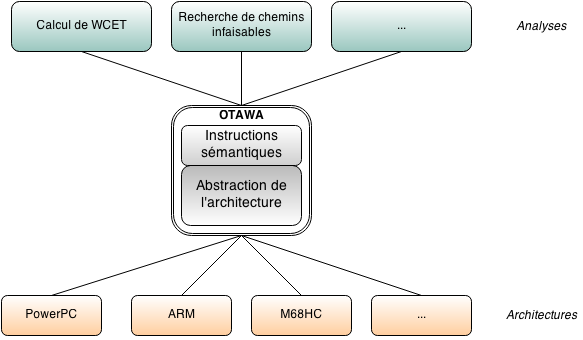
\includegraphics[width=\textwidth]{pictures/otawa_abstraction_architecture.png}
    \caption{OTAWA permet aux analyses de s'abstraire de l'architecture}
    \label{abstraction architecture}
  \end{figure}

  Voici, sans donner plus de détails pour le moment, à quoi ressemble la traduction de code assembleur (celui-ci a été généré avec gcc) en instructions sémantiques. Les \texttt{tX} sont des variables temporaires utilisées pour la traduction en instructions sémantiques et les \texttt{?X} sont les registres. Pour chaque instruction assembleur, on trouve dessous une ou plusieurs instructions sémantiques équivalentes, en commentaire :

  \begin{lstlisting}[language={[ARM]Assembler}]
    ldr r0, [pc, #20]
    @	seti ?15, 0x8310
    @	seti t2, 0x14
    @	add t1, ?15, t2
    @	load ?0, t1, uint32

    mov r1, #0
    @	seti ?1, 0x0

    mov r2, r1
    @	set t1, ?1
    @	set ?2, t1

    bl 8574
    @	seti t1, 0x8574
    @	seti ?14, 0x8318
    @	branch t1
  \end{lstlisting}

  De plus amples explications à ce sujet seront données dans la suite de ce mémoire.

  \subsection{Restrictions}
  Nous travaillons dans le cadre de cette étude exclusivement sur des programmes sans boucles. Le problème de la gestion des boucles est un problème complexe qui ne pouvait pas se traiter en l'espace de quelques mois. Cette hypothèse n'est pas complètement irréaliste puisqu'il existe des programmes, voire même des langages sans boucles. Plus tard quand ce travail sera continué en thèse, il faudra les traiter mais nous ne savons pas encore à quel point ce traitement sera limité en efficacité.

  Un autre vaste problème se pose, celui de la gestion de la mémoire. Il s'agit de se représenter dans le programme l'état de la mémoire (ou du moins les quelques parties sur lesquelles on sait quelque chose) et de déduire des propriétés sur la valeur du registre de destination d'un LOAD en mémoire. Le traitement des instructions mémoire est à l'heure que j'écris ces lignes quasiment terminé mais il reste assez limité.

  Notre programmme ne traite pour l'instant pas les instructions sémantiques d'OTAWA spécifiques aux ``unsigned'' (entiers représentés non signés). En effet, pour une même valeur binaire dans un registre, selon qu'on l'interprète comme un entier signé ou non, son interprétation peut être différente. Un exemple sur 4 bits est donné sur la figure~\ref{representation_signed_unsigned}.

  \begin{figure}
    \centering
    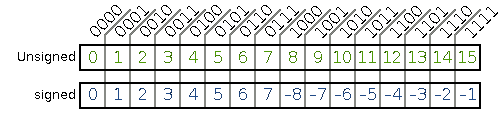
\includegraphics[width=250px]{pictures/representation_signed_unsigned.png}
    \caption{Différentes interprétations de la valeur d'un registre}
    \label{representation_signed_unsigned}
  \end{figure}

  Toutefois, l'interprétation de la valeur d'un registre est identique tant que le bit de poids fort est à 0, c'est à dire tant que la valeur interprétée appartient à l'intervalle $\llbracket0, 2^{n-1}-1\rrbracket$, où $n$ est le nombre de bits du registre.

  Et bien sûr, toutes les instructions qui ne sont pas supportées par OTAWA (impossibles à traduire en expression sémantiques) ne sont pas non plus supportées par notre programme, même si ce type d'erreur est géré de manière à ne pas être critique : on va perdre de l'information et donc peut-être détecter moins de chemins infaisables, mais l'analyse n'échoue pas.

  \newpage{}
  \section{Contexte}
  \subsection{Choix du solveur SMT}
  Pour le choix de notre solveur SMT, nous avons dressé un petit état de l'art en nous basant principalement sur des résultats de la SMT-COMP~\cite{SMT-COMP}, une compétition entre solveurs, en éliminant d'office les solveurs qui ne présentaient pas d'API utilisable en C++ :

  \begin{itemize}
    \item Z3~\cite{smt_z3}
    \begin{itemize}
      \item Gagnant de la SMT-COMP 2011
      \item Apparemment encore le plus performant en termes de temps d'exécution
      \item Développé par Microsoft Research
      \item Distribué sous la licence \textit{Microsoft Research License Agreement Non-Commercial Use Only}
    \end{itemize}
    \item CVC4~\cite{smt_cvc4}
    \begin{itemize}
      \item CVC3 a l'air insuffisant et limité mais le solveur a été globalement réécrit pour CVC4, bien qu'il semble y avoir une certaine continuité dans les \textit{features} proposées
      \item CVC4 a tourné sur de multiples benchmarks et a toujours eu de bons ou très bons résultats
      \item Open source, sans restriction pour un usage commercial ou à fins de recherches
    \end{itemize}
    \item MathSAT 5~\cite{smt_mathsat5}
    \begin{itemize}
      \item API disponible seulement en C
      \item Bons résultats pour MathSAT5-smtcomp12
      \item ``An SMT solver for Formal Verification'', ouverture possible sur la vérification formelle
    \end{itemize}
    \item Boolector~\cite{smt_boolector}
    \begin{itemize}
      \item API disponible seulement en C
      \item Quelques très bons résultats à la SMT-COMP mais qui ne semblent pas porter sur des critères intéressants pour notre usage.
    \end{itemize}
    \item SONOLAR~\cite{smt_sonolar}
    \begin{itemize}
      \item Modeste dans ses performances
      \item N'a été testé que sur benchmarks notés ``BV'', restrictions aux booléens ?
    \end{itemize}
    \item MISTRAL~\cite{smt_mistral}
    \begin{itemize}
      \item Pas évalué à la SMT-COMP 2012
    \end{itemize}
    \item VeriT~\cite{smt_verit}
    \begin{itemize}
      \item Pas évalué à la SMT-COMP 2012
    \end{itemize}
    \item Barcelogic~\cite{smt_barcelogic}
    \begin{itemize}
      \item Pas évalué à la SMT-COMP 2012
    \end{itemize}
  \end{itemize}

  \begin{wrapfigure}{R}{1.5in}
    \centering
    
\includegraphics{./pictures/cvc4.png}
    % cvc4.png: 300x168 pixel, 300dpi, 2.54x1.42 cm, bb=0 0 72 40
    \label{cvc4}
  \end{wrapfigure}

  Notre choix s'est finalement porté sur \textbf{CVC4}, pour ses bonnes performances, son API riche et bien documentée, et sa licence très libre.

  Notre application utilise toutefois ses propres structures pour manipuler les prédicats, et le module qui fait l'interface avec le solveur SMT devrait être suffisamment indépendant du reste pour permettre de changer de solveur SMT si besoin sans trop de difficultés.

  \subsection{Représentation en graphe de flot de contrôle}
  Lors de notre analyse, nous considérerons le programme sous la forme d'un graphe connexe enraciné, appelé \textbf{graphe de flot de contrôle, ou CFG} (Control Flow Graph). Dans le cas des programmes sans boucles que nous traitons, il s'agit aussi d'un graphe acyclique.

  Un CFG est donc un graphe dont les noeuds sont appelés des \textbf{blocs de bases}, et qui sont constitués d'une suite d'instructions exécutées \textit{séquentiellement}. Il ne peut donc y avoir d'appels de fonctions, de conditions, de boucles, ou tout autre branchement à l'intérieur d'un bloc de base (excepté en dernière instruction). La figure~\ref{bloc de base} en montre un exemple.

  \begin{figure}
    \centering
    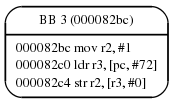
\includegraphics[scale=0.5]{pictures/basicblock.png}
    % basicblock.png: 173x104 pixel, 72dpi, 6.10x3.67 cm, bb=0 0 173 104
    \caption{Un exemple de bloc de base en langage machine ARM}
    \label{bloc de base}
  \end{figure}

  Les arêtes représentent les chemins d'exécution du programme, elles correspondent à des branchements où à l'exécution séquentielle du programme. Il y a deux types de branchements : les branchements conditionnels et les branchements inconditionnels.

  Parmi les \textbf{branchements conditionnels}, ceux qui correspondent à l'arc ``pris'', c'est-à-dire au cas où la condition évoquée est vérifiée, sont annotés sur le CFG avec l'étiquette ``\textit{taken}'', l'arc dit ''non pris'' n'a conventionellement pas d'étiquette.

  Parmi les \textbf{branchements inconditionnels}, il peut s'agir de l'exécution séquentielle du programme ou d'un branchement non conditionnel (ce qui revient en assembleur à changer le registre pointeur d'instruction \texttt{pc} ou \texttt{r15} pour l'ARM) auquel cas l'arc n'est pas annoté, ou il peut s'agir d'un appel de fonction (\textit{Branch with Link} en assembleur), auquel cas l'arc est dessiné en pointillés et annoté ``\textit{call}''.

  Les figures \ref{branchement conditionnel} et \ref{branchement inconditionnel} montrent des exemples de ces branchements.

  \begin{figure}
    \begin{minipage}[c]{.46\linewidth}
      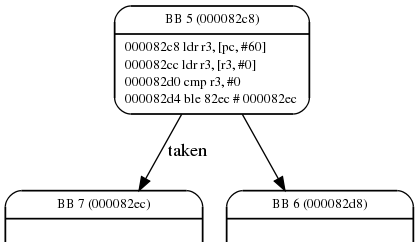
\includegraphics[scale=0.5]{./pictures/conditional_branch.png}
      % conditional_branch.png: 419x248 pixel, 96dpi, 11.08x6.56 cm, bb=0 0 314 186
      \caption{Exemples de branchements conditionnels}
      \label{branchement conditionnel}
   \end{minipage} \hfill
   \begin{minipage}[c]{.46\linewidth}
      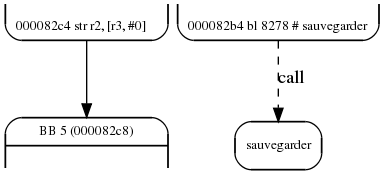
\includegraphics[scale=0.5]{./pictures/incoditional_branch.png}
      % incoditional_branch.png: 423x181 pixel, 96dpi, 11.19x4.79 cm, bb=0 0 317 136
      \caption{Exemples de branchements inconditionnels}
      \label{branchement inconditionnel}
   \end{minipage}
\end{figure}

  \bigbreak

  Prenons pour exemple l'algorithme~\ref{alg:1} que nous avions présenté plus haut. Le CFG en pseudo-code correspondant est exhibé sur la figure~\ref{cfg}. On y voit bien apparaître les 4 chemins cités précédemment. %TOLDO: vérifier que l'algo soit bien présent *plus haut*

  La figure~\ref{cfg_genere} montre le CFG généré par OTAWA à partir du code ARM correspondant à l'algorithme~\ref{alg:1} (compilé à partir d'un fichier C). On y observe à peu près la même structure que sur le CFG en pseudo-code, avec des calls à la fonction \texttt{sauvegarder} et des instructions ARM plus volumineuses à l'intérieur des blocs.

  \begin{figure}
    \centering
    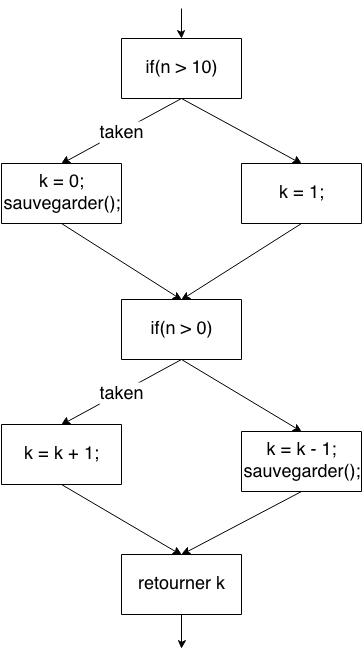
\includegraphics[height=330px]{pictures/cfg.png}
    \caption{CFG de l'algorithme~\ref{alg:1}}
    \label{cfg}
  \end{figure}

  \begin{figure}
    \centering
    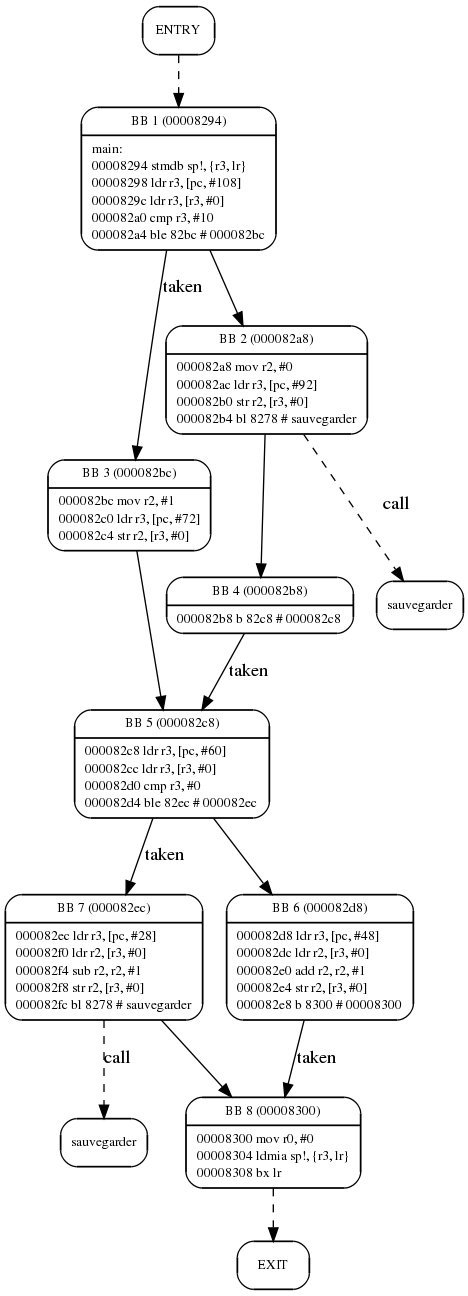
\includegraphics[height=525pt]{pictures/cfg_genere.png}
    % cfg_genere.png: 468x1296 pixel, 72dpi, 16.51x45.72 cm, bb=0 0 468 1296
    \caption{CFG généré par OTAWA}
    \label{cfg_genere}
  \end{figure}
  
  \newpage{} % TOLDO: maybe remove this
  \subsection{Les instructions sémantiques d'OTAWA} 
 
  \begin{figure}
    \begin{tabular}{|l|l|} \hline
      \textbf{Instruction} & \textbf{Sémantique}\\ \hline \hline
      \texttt{NOP} & (rien)\\ \hline
      \texttt{BRANCH} & \\
      \texttt{TRAP} & Indicateurs du flot du programme\\
      \texttt{CONT} & \\ \hline
      \texttt{IF cond sr jump} & si la condition \texttt{cond} sur le registre \texttt{sr} est vraie, continuer,\\
      & sinon sauter \texttt{jump} instructions\\ \hline
      \texttt{LOAD reg addr type} & reg $\leftarrow$ \texttt{MEM\textsubscript{type}} \\ \hline
      \texttt{STORE reg addr type} & \texttt{MEM\textsubscript{type}} $\leftarrow$ \texttt{reg}\\ \hline
      \texttt{SCRATCH d} & \texttt{d $\leftarrow$ $\top$} \textit{(invalidation)}\\ \hline
      \texttt{SET d a} & \texttt{d $\leftarrow$ a}\\ \hline
      \texttt{SETI d cst} & \texttt{d $\leftarrow$ cst}\\ \hline
      \rowcolor{Gray} \texttt{SETP d cst} & \texttt{page(d) $\leftarrow$ cst}\\ \hline
      \texttt{CMP d a b} & \texttt{d $\leftarrow$ a $\sim$ b}\\ \hline
      \rowcolor{Gray} \texttt{CMPU d a b} & \texttt{d $\leftarrow$ a $\sim$\textsubscript{unsigned} b}\\ \hline
      \texttt{ADD d a b} & \texttt{d $\leftarrow$ a $+$ b}\\ \hline
      \texttt{SUB d a b} & \texttt{d $\leftarrow$ a $-$ b}\\ \hline
      \rowcolor{Gray} \texttt{SHL d a b} & \texttt{d $\leftarrow$ unsigned(a) <{<} b}\\ \hline
      \rowcolor{Gray} \texttt{SHR d a b} & \texttt{d $\leftarrow$ unsigned(a) >{>} b}\\ \hline
      \texttt{ASR d a b} & \texttt{d $\leftarrow$ a >{>} b}\\ \hline
      \texttt{NEG d a} & \texttt{d $\leftarrow$ $-$a}\\ \hline
      \rowcolor{Gray} \texttt{NOT d a} & \texttt{d $\leftarrow$ $\neg$a}\\ \hline
      \rowcolor{Gray} \texttt{AND d a b} & \texttt{d $\leftarrow$ a \& b}\\ \hline
      \rowcolor{Gray} \texttt{OR d a b} & \texttt{d $\leftarrow$ a | b}\\ \hline
      \rowcolor{Gray} \texttt{XOR d a b} & \texttt{d $\leftarrow$ a $\oplus$ b}\\ \hline
      \texttt{MUL d a b} & \texttt{d $\leftarrow$ a $\times$ b}\\ \hline
      \rowcolor{Gray} \texttt{MULU d a b} & \texttt{d $\leftarrow$ unsigned(a) $\times$ unsigned(b)}\\ \hline
      \texttt{DIV d a b} & \texttt{d $\leftarrow$ a / b}\\ \hline
      \rowcolor{Gray} \texttt{DIVU d a b} & \texttt{d $\leftarrow$ unsigned(a) / unsigned(b)}\\ \hline
      \texttt{MOD d a b} & \texttt{d $\leftarrow$ a \% b}\\ \hline
      \rowcolor{Gray} \texttt{MODU d a b} & \texttt{d $\leftarrow$ unsigned(a) \% unsigned(b)}\\ \hline
      \rowcolor{Gray} \texttt{SPEC} & (instruction spéciale non supportée par OTAWA)\\ \hline
    \end{tabular}
    \textit{En gris : les instructions qui ne sont pas (encore) traitées par notre analyse.}
    \label{seminsts}
    \caption{Liste des instructions sémantiques d'OTAWA}
  \end{figure}
  
  \'Etant donné que les systèmes temps-réels embarqués tournent sur des architectures très différentes, OTAWA fournit une abstraction de la sémantique des instructions machine, nous l'avions déjà évoqué au chapitre 1.3. %TOLDO
  
  Ce langage, présenté sur la figure~\ref{seminsts} est composé d'instructions simplifiées de type RISC qui utilisent des registres machine ou des variable temporaires. \'Etant donné sa simplicité par rapport aux assembleurs réels, la plupart de leurs instructions sont traduites par un bloc d'instructions sémantiques. Le langage sémantique définit des registres temporaires $t_0, ..., t_n$ dont la durée de vie est limitée à un bloc d'instructions sémantiques (correspondant à une seule instruction assembleur), et qui ne servent qu'à passer des valeurs entre les différentes instructions sémantiques du bloc.
  
  Nous distinguons donc deux types de variables :
  
  \begin{itemize}
    \item les registres machine, notés $r_0$, $r_1$, ..., $r_n$ ou parfois $?0, ?1, ?n$, qui sont permanentes ;
    \item les variables temporaires, notées $t_1$, $t_2$, ..., $t_n$, qui sont locales à un bloc.
  \end{itemize}
  
  Décortiquons l'exemple précédemment utilisé :
  
  \begin{lstlisting}[language={[ARM]Assembler}]
    mov r1, #0
    @	seti ?1, 0x0
  \end{lstlisting}
  
  Ici, on a une instruction machine assez basique qui peut être traduite en une seule instruction sémantique. \texttt{mov r1, \#0} correspond à ``mettre la valeur 0 dans le registre $r_1$'', ce qui s'écrit en instructions sémantique comme \texttt{seti, ?1, 0x0}.

  \begin{lstlisting}[language={[ARM]Assembler}]
    mov r2, r1
    @	set t1, ?1
    @	set ?2, t1
  \end{lstlisting}
  
  Cette fois-ci c'est un peu plus compliqué puisque nous faisons à la fois la lecture d'un registre et l'écriture dans un registre : nous avons besoin de deux instructions sémantiques pour traduire ce que fait ``\texttt{mov r2, r1}'', c'est-à-dire ``mettre dans $r_2$ la valeur de $r_1$'', nous utilisons donc une variable temporaire ($t_1$) qui fait l'intermédiaire. La première instruction lit le registre $r_1$, la deuxième écrit dans le registre $r_2$.

  \begin{lstlisting}[language={[ARM]Assembler}]
    bl 8574
    @	seti t1, 0x8574
    @	seti ?14, 0x8318
    @	branch t1
  \end{lstlisting}

  Il s'agit ici d'un branchement avec lien (on se souvient d'où on a fait l'appel de fonction pour y revenir quand la fonction se termine). Techniquement, cela se traduit par un simple branchement avec la sauvegarde au préalable de l'adresse de la prochaine instruction dans $r_{14}$ (on l'appelle aussi le registre \textit{link}).
  
  OTAWA génère donc une première instruction sémantique qui écrit l'adresse sur laquelle brancher (c'est-à-dire, là où il faut aller, le début de la fonction) qui est fournise en paramètre de \texttt{bl} (ici, \texttt{0x8574}). La deuxième instruction sémantique s'occupe de mettre l'adresse de la prochaine instruction machine dans $r_14$ (ici, \texttt{0x8318}). Enfin, nous faisons le branchement sur $t_1$ avec \texttt{branch t1}.
  
  Nous nous désintéressons complètement au fonctionnement de cette traduction, qui est expliqué plus en détail dans cet article de H. Cassé, F. Birée et P. Sainrat~\cite{otawa}, puisque nous ne travaillerons dans le cadre de notre analyse qu'avec les instructions sémantiques fournies par OTAWA.
  
  \subsection{Interprétation abstraite}
  Il s'agit maintenant d'introduire brièvement la théorie derrière notre travail, l'interprétation abstraite~\cite{cousot}.
  
  Une quadruplet  $(L, \alpha, \gamma, M)$, composé deux domaines et deux fonctions, un domaine concret $L$, un domaine abstrait $M$, une fonction d'abstraction $\alpha : L \rightarrow M$ et une fonction de concrétisation $\gamma : M \rightarrow L$, est une \textit{correspondance de Galois}~\cite{nielson} si elle respecte les deux propriétés suivantes :
  
  \begin{align}
    \gamma \circ \alpha \sqsupseteq id_L\\
    \alpha \circ \gamma \sqsubseteq id_M
  \end{align}

  où $id_L$ et $id_M$ sont les fonctions d'identité respectives de $L$ et $M$.
  
  Regardons tout de suite un exemple pour mieux comprendre : prenons $L \coloneqq \mathscr{P}(\mathds{Z})$, $M \coloneqq \{\perp, +, -\}$, et
  
  \begin{align*}
    \alpha (l) \coloneqq \left\{ 
    \begin{array}{ll}
      + & \si\ l \subseteq \mathds{Z}_{\geq 0}\\
      - & \si\ l \subseteq \mathds{Z}_{< 0}\\
      \perp & \sinon\
    \end{array} \right.
  \end{align*}
  
  \begin{align*}
    \gamma (m) \coloneqq \left\{ 
    \begin{array}{ll}
      \llbracket 0, +\infty\llbracket & \si\ m = -\\
      \rrbracket -\infty, -1\rrbracket & \si\ m = +\\
      \rrbracket -\infty, +\infty\llbracket  & \si\ m =\ \perp\\
    \end{array} \right.
  \end{align*}
  
  ``$\sqsupseteq$'' correspond ici à ``$\supseteq$'' et ``$\sqsubseteq$'' à ``$=$'' dans $M$. Essayons maintenant de vérifier que $(L, \alpha, \gamma, M)$ est une correspondance de Galois :
  
  \begin{align*}
    \gamma \circ \alpha (l) = \left\{ 
    \begin{array}{ll}
      \llbracket 0, +\infty\llbracket & \si\ l \subseteq \mathds{Z}_{\geq 0}\\
      \rrbracket -\infty, -1\rrbracket & \si\ l \subseteq \mathds{Z}_{< 0}\\
      \rrbracket -\infty, +\infty\llbracket & \sinon\
    \end{array} \right.
  \end{align*}
  
  Or,
  
  \begin{align*}
    \forall l \subseteq \mathds{Z}_{\geq 0},\ & \llbracket 0, +\infty\llbracket \supseteq l\\
    \forall l \subseteq \mathds{Z}_{< 0},\    & \rrbracket -\infty, -1\rrbracket \supseteq l\\
    \forall l \in \mathscr{P}(\mathds{Z}),\   & \rrbracket -\infty, +\infty\llbracket \supseteq l
  \end{align*}
  
  Donc $\forall l \in L, \gamma \circ \alpha (l) \supseteq l = id_L(l)$. Donc la propriété $(1)$ est bien respectée.
  La deuxième propriété est plus rapide à vérifier, nous allons donc la détailler un peu :
  
  \begin{align*}
    \alpha \circ \gamma (m)\ &=\ \left\{ 
    \begin{array}{ll}
      \alpha (\llbracket 0, +\infty\llbracket) & \si\ m = -\\
      \alpha (\rrbracket -\infty, -1\rrbracket) & \si\ m = +\\
      \alpha (\rrbracket -\infty, +\infty\llbracket)  & \si\ m =\ \perp\\
    \end{array} \right.\\
    &= \ \left\{ 
    \begin{array}{ll}
      - & \si\ m = -\\
      + & \si\ m = +\\
      \perp  & \si\ m =\ \perp\\
    \end{array} \right.\\
    &= m
  \end{align*}
  
  Donc $\forall m \in M, \alpha \circ \gamma (m) = m = id_M(m)$. Donc la propriété $(2)$ est bien repectée.
  
  $(L, \alpha, \gamma, M)$ est donc bien une correspondance de Galois. \hfill $\blacksquare$
  
  \bigbreak
  
  Il existe d'autres approches plus visuelles et moins algébriques des correspondances de Galois. Prenez la fleur 1 à gauche de la figure ci-dessous, par exemple, que nous appelerons $l$ :
  
  
  \begin{center}
    \begin{minipage}{.3\textwidth}
      \begin{center}
	
\includegraphics[scale=0.19]{./pictures/flower2.png}\\
	% flower2.png: 604x788 pixel, 96dpi, 15.98x20.85 cm, bb=0 0 453 591
	\textsc{fleur 1}
      \end{center}
    \end{minipage}
    \begin{minipage}{.3\textwidth}
      \begin{center}
	
\includegraphics[scale=0.19]{pictures/flower4.png}\\
	\textsc{fleur 2}
      \end{center}
    \end{minipage}
    \begin{minipage}{.3\textwidth}
      \begin{center}
	
\includegraphics[scale=0.19]{./pictures/flower3.png}\\
	\textsc{fleur 3}
      \end{center}
    \end{minipage}
  \end{center}
  
  Considérons que le domaine concret ($L$) est l'ensemble des dessins sur le plan ($l \in L$), et que le domaine abstrait ($M$) ne contient que des contours.
  
  La fonction d'abstraction $\alpha\ : L \rightarrow M$ ne retient que les contours du dessin. Par exemple, sur la figure ci-dessus, la fleur 2 est $\alpha (l)$.

  La fonction de concrétisation $\gamma\ : M \rightarrow L$ remplit le dessin, de telle manière que $\gamma \circ \alpha (l)$  soit la fleur 3.
  
  On se rend compte que la première propriété $(1)$ pour que $(L, \alpha, \gamma, M)$ soit une correspondance de Galois est respectée pour $l$, puisqu'on a $\gamma \circ \alpha (l) \sqsupset l$ (le dessin de la fleur 3 ``contient'' la fleur 1).
  
  \medbreak
  
  La deuxième propriété est assez triviale, puisque lorsqu'on prend un contour $m$ (comme sur la fleur 2 ci-dessus), qu'on le concrétise (on le ``remplit'') pour obtenir $\gamma (m)$ (fleur 3) et qu'on revient dans le monde abstrait, avec $\alpha \circ \gamma (m)$ fleur 2), on obtient toujours l'identité ($id_M$).
  
  $\alpha \circ \gamma$ est donc \textit{égal} à $id_M$, et à fortiori la condition $(2)$ est respectée ($\alpha \circ \gamma \sqsubseteq id_M$). Nous n'avons montré ces propriétés que sur un exemple, celui de la fleur $l$, nous n'avons donc rien prouvé (ce n'est pas l'objet) mais nous avons déjà donné quelques éléments d'intuition.
  
  \bigbreak
  
  Quel intérêt pour l'analyse d'un programme ? Nous voulons trouver des chemins infaisables dans un programme, dont l'état initial est schématisé par la fleur 1.
  
  Dans la métaphore, cela revient, par exemple, à vérifier que le dessin ne disparait jamais entièrement (il n'est jamais vide) au fur et à mesure de l'exécution du programme. Pour cela, nous nous représentons l'état du programme, une abstraction de la réalité, la fleur 2.
  
  Nous suivons le fil d'exécution du programme, en appliquant à notre état abstrait (notre contour) les modifications subies par le programme, c'est-à-dire la lecture d'instructions. Par exemple, nous lisons une instruction qui fait, dans notre métaphore, pivoter la fleur de 90$^{\circ}$ (fleur 4 ci-dessous) :  
  
  \begin{center}
    \begin{minipage}{.45\textwidth}
      \begin{center}
	
\includegraphics[scale=0.19]{./pictures/flower5.png}\\
	% flower5.png: 788x604 pixel, 96dpi, 20.85x15.98 cm, bb=0 0 591 453
	\textsc{fleur 4}
      \end{center}
    \end{minipage}
    \begin{minipage}{.45\textwidth}
      \begin{center}
	
\includegraphics[scale=0.19]{./pictures/flower6.png}\\
	% flower6.png: 788x604 pixel, 96dpi, 20.85x15.98 cm, bb=0 0 591 453
	\textsc{fleur 5}
      \end{center}
    \end{minipage}
  \end{center}
  
  Pour que notre analyse reste juste, il faut que notre état abstrait reste une surapproximation de la réalité (c'est-à-dire ici que le dessin concrétisé contient toujours le dessin obtenu en faisant les modifications à l'original), comme sur la fleur 5.
  
  Comme on surestime grâce à la propriété $(1)$ de la correspondace de la Galois ($\gamma \circ \alpha \sqsupset id_L$), il se peut qu'on ne détecte pas certains chemins infaisables (c'est-à-dire des disparitions du dessin), en revanche \textbf{on ne peut pas trouver de chemins infaisables faux} (c'est-à-dire notre dessin ne disparaîtra pas sans raison), et c'est là l'essentiel : en analyse statique, on abstrait des domaines complexes en domaines plus simples en faisant des surestimations, on peut manquer des propriétés mais on ne peut pas en trouver de fausses.
  
  Par exemple, nous lisons des instructions qui nous demandent maintenant de supprimer la tige (fleur 6) :
  
  \begin{center}
    \begin{minipage}{.3\textwidth}
      \begin{center}
	
\includegraphics[scale=0.19]{./pictures/flower7.png}\\
	% flower7.png: 788x604 pixel, 96dpi, 20.85x15.98 cm, bb=0 0 591 453
	\textsc{fleur 6}
      \end{center}
    \end{minipage}
    \begin{minipage}{.3\textwidth}
      \begin{center}
	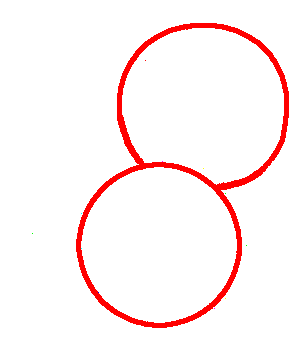
\includegraphics[scale=0.19]{./pictures/flower8.png}\\
	\textsc{fleur 7}
      \end{center}
    \end{minipage}
    \begin{minipage}{.3\textwidth}
      \begin{center}
	
\includegraphics[scale=0.19]{./pictures/flower9.png}\\
	\textsc{fleur 8}
      \end{center}
    \end{minipage}
  \end{center}
  
  puis de supprimer toutes les pétales une à une, jusqu'à arriver à la fleur 7, et enfin à la fleur 8.
  
  Il s'agit là d'un exemple de chemin infaisable que nous n'avons pas pu trouver à cause de notre surestimation (dans la réalité, ce rond restant correspond au ``noyau'' vide de la fleur 1, et le dessin a donc disparu).
  
  \bigbreak
  
  Dans notre travail, au lieu d'abstraire les contours d'un dessin, nous allons abstraire l'état de l'exécution du programme dans la machine à un moment donné par une liste de prédicats. Il faut garder en tête que cette représentation du programme sera imprécise et surestimée, mais que nous resterons toujours correct.
  
  
  
% Cela explique le fonctionnement du invalidate().
% NOTE: soit S l'ens des états du programme et S' = { s in S \ (P1 /\ P2 /\ P3) s = T }, les prédicats induisent un sous-ensemble des états et il est facile de voir que S" = { s in S \ (P1 /\ P2) s = T } inclus S'.
% En fait, on peut voir un prédicat comme une fonction P: S -> Bool
% De plus, un ensemble de prédicats insatisfiable, Ps donnerait un ensemble d'état vide { } montrant par là qu'il n'existe aucun chemin d'exécution permettant d'atteindre ce point du programme.
  
  \newpage{}
  \section{Algorithme de recherche de chemins infaisables}  
  \subsection{Représentation des prédicats}
  Nous utilisons nos propres structures de prédicats, appropriées à l'usage qui leur est destiné. En voici la grammaire abstraite :

  Un prédicat est composé de deux opérandes et d'un opérateur de comparaison :
  
  \begin{algorithm}[H]
    \textbf{Prédicat}: Expression \texttimes~Comparateur \texttimes~Expression\\
        \textbf{Comparateur}:\\
            \qquad |\quad EQ, // $=$\\
            \qquad |\quad NE, // $\neq$\\
            \qquad |\quad LE,\, // $\leq$\\
            \qquad |\quad LT\: // $<$\\
  \end{algorithm}
  
  Pour limiter le nombre de cas à traiter, nous n'avons pas inclus les opérateurs $>$ et $\geq$ (on peut les retrouver en inversant l'ordre des opérandes avec $<$ et $\leq$). Ce genre d'astuce est aussi utilisé dans l'API fournie par le solveur SMT CVC4, à cela près qu'ils préfèrent exclure $\leq$ et $<$.
  
  Une expression peut être une constante, une variable, une valeur en mémoire, ou une expression arithmétique composée d'un opérateur arithmétique et de deux opérandes, elles-mêmes des expressions :

  \begin{algorithm}[H]
        \textbf{Expression}:\\
            \qquad |\quad Const(k: $\mathds{Z}$)\\
            \qquad |\quad Var(id: Variable)\\
            \qquad |\quad Mem(addr: Adresse)\\
            \qquad |\quad \-- Expression\\
            \qquad |\quad Expression + Expression\\
            \qquad |\quad Expression \--\ Expression\\
            \qquad |\quad Expression \texttimes\ Expression\\
            \qquad |\quad Expression / Expression\\
            \qquad |\quad Expression \textit{mod} Expression\\
  \end{algorithm}
  
  Nous ne supportons pour le moment que les opérations sur les entiers signés ($\mathds{Z}$), donc pas d'opérateurs ``non signés'' (sur $\mathds{N}$), ou d'opérateurs logiques (sur $\mathds{Z}/$\raisebox{-0.5ex}{$2\mathds{Z}$}), comme \texttt{ET}, \texttt{OU} et \texttt{NON}.
  
  Une variable peut être un registre temporaire (un entier strictement positif) ou un registre (un entier positif). La quantité de registres est généralement très limitée mais comme nous travaillons indépendemment de l'architecture, nous ne pouvons pas connaître cette limitation (et nous n'en avons pas besoin).

  \begin{algorithm}[H]
        \textbf{Variable}:\\
            \qquad |\quad Temporaire(k: $\mathds{N^*}$)\\
            \qquad |\quad Registre(k: $\mathds{N}$)\\
  \end{algorithm}
  
  Une adresse peut être absolue (par exemple, \texttt{0x8014}), ou relative à une variable (par exemple \texttt{r13 + 4}).
  
  \begin{algorithm}[H]
        \textbf{Adresse}:\\
            \qquad |\quad Absolu(k: $\mathds{Z}$)\\
            \qquad |\quad Relatif(reg: Registre, offset: $\mathds{Z}$)\\
  \end{algorithm}

  \bigbreak

%OKHUG: pas de représentation du ET, OU, NON logiques ? Expliquer pourquoi.

  A chaque prédicat nous lui associerons un arc du CFG, qui correspondra, sur le chemin emprunté, à l'arc immédiatement après le bloc de base qui contenait l'instruction qui a généré le prédicat en question.
  
  Nous ne transportons donc pas exactement une liste de prédicats (qui correspond à une conjonction de prédicats), mais plutôt une liste de couples \texttt{(Prédicat, Edge)} qui contiennent des informations sur l'origine de leur prédicats. Cela nous permettra ensuite, une fois que nous aurons trouvé une insatisfiabilité, de remonter jusqu'aux arêtes responsables du CFG et d'identifier le chemin infaisable. Par exemple, à partir de la liste :
  
  \[\{(x = 0)^{1\rightarrow 2}, (y = x)^{3\rightarrow 5}, (y > 10)^{3\rightarrow 5} \}\]
  
  on pourra en déduire que le chemin qui passe par les arcs $\{1\rightarrow 2, 3\rightarrow 5\}$ est infaisable.
  
  \subsection{Analyse d'un graphe de flot de contrôle}
  Comme nous travaillons sans boucles, l'algorithme ci-dessous n'est pas correct, ou du moins ne terminera pas si on le fait fonctionner sur un CFG avec boucles. Nous initialisons d'abord l'algorithme de parcours de graphe de contrôle avec le premier bloc de base du CFG, qui nous est donné par OTAWA.

  Voici donc l'algorithme en pseudo-code, qui prend en paramètre un bloc de base :\\

   % http://www.cs.toronto.edu/~frank/Useful/algorithm2e.pdf
  \begin{algorithm}[H]
    % \caption{analyzeBasicBlock}
    \Donnees{bb: BasicBlock, lpreds: LabelledPredicate list}
    \Res{Chemins infaisables trouvés}
    \Si{bb est un bloc de sortie (EXIT)}{
        \Retour{[]} // Fin de l'analyse de ce chemin
    }
    Appeler le solveur SMT avec lpreds;\\
    \Si{on a trouvé une insatisfiabilité}{
	Extraire la liste des chemins infaisables;\\
	\Retour{cette liste} // Fin de l'analyse de ce chemin
    }
    preds = parseBasicBlock(bb); // Analyse linéaire des instructions sémantiques\\
    \Pour{tous les arcs sortants edge de bb}{
	Labeller les prédicats preds avec l'arc edge comme étiquette;\\
	Ajouter ces prédicats labellés à lpreds;\\
	Appel récursif de cette fonction avec pour paramètres (\\
	    \pushline le bloc de base vers lequel edge pointe,\\
	    la nouvelle liste lpreds\\
	\popline);\\
    }
  \end{algorithm}
  

  \subsection{Analyse des instructions sémantiques d'un bloc de base}
  Le programme parcourt les blocs de base linéairement en mettant à jour la liste de prédicats.

  Nous définissons d'abord une fonction d'invalidation d'une variable dans la liste de prédicats, qui consiste à supprimer tous les prédicats qui utilisent cette variable. En effet, nous allons rencontrer des instructions ``destructrices'', c'est-à-dire des instructions qui vont rendre invalides toutes les propriétés que nous avions sur la variable en question. Par exemple, si nous rencontrons une instruction qui met \texttt{r0} à \texttt{0}, alors il faudra supprimer les prédicats précédemment créés \texttt{r0 = r1} et \texttt{r0 = 2}.

  \begin{lstlisting}[mathescape]
    invalidate var p =
        {predicate $\in$ p $|$ var $\notin$ predicate}
  \end{lstlisting}

  Les seules fois où l'invalidation ne sera pas nécessaire pour une instruction qui modifie une variable seront celles où la modification en question est \textbf{bijective}. Par exemple, une instruction qui incrémente une variable de \texttt{1} (abstraite par la fonction $\textit{ajouter}_1$ ici) est bijective :
%OKHUG: bijective me fait bizarre dans ce contexte. Inversible peut-être ?

  \begin{align*}
    \textit{ajouter}_1 : \mathds{Z} &\bijmap \mathds{Z}\\
    x &\mapsto x+1
  \end{align*}
  \begin{align*}
    \textit{ajouter}_1^{-1} : \mathds{Z} &\bijmap \mathds{Z}\\
    x &\mapsto x - 1
  \end{align*}

  Si par exemple nous rencontrons une instruction qui nous demande d'incrémenter de \texttt{1} la variable \texttt{r0}, nous pourrons simplement remplacer \texttt{r0} par \texttt{r0~-~1} dans les prédicats \texttt{r0 = r1} et \texttt{r0 = 2}. Nous obtenons les nouveaux prédicats \texttt{r0 - 1 = r1} et \texttt{r0 - 1 = 2} (c'est-à-dire \texttt{r0 = 3}).
  
  Nous avons également implémenté des stratégies pour essayer de préserver l'information autant que possible lors de l'invalidation d'une variable. Par exemple, si on a un prédicat \texttt{r0 = r1} et que l'on doit invalider \texttt{r0}, on se contentera de supprimer ce premier prédicat et remplacer toutes les occurences de \texttt{r0} par \texttt{r1}.
  
  Il faut bien voir que nous avons la liberté de perdre autant d'informations (c'est-à-dire de supprimer des prédicats) que nous le voulons sur l'état du programme. Par exemple, si on a $\{p_1, p_2, p_3\}$ (c'est-à-dire $p_1 \land p_2 \land p_3$), on peut enlever n'importe quel prédicat $p_1$, $p_2$ ou $p_3$ et garder un résultat valide : on a juste perdu de la précision.

  \bigbreak

  Il s'agit maintenant de définir l'effet de la lecture de chaque instruction sur la liste de prédicats.
  Exemple sur un premier cas trivial :

  \begin{lstlisting}
    t [NOP] p =
        p (* rien ne change *)
  \end{lstlisting}

  La fonction de traduction \texttt{t} opère sur une instruction (ici \texttt{NOP}) et la liste de prédicats \texttt{p}.

  Regardons maintenant comment est traitée l'instruction d'assignation d'une variable à une autre variable (\texttt{SET}) :

  \begin{lstlisting}
    t [SET d a] p =
        (d = a) @ (invalidate d p)
  \end{lstlisting}

  Un nouveau prédicat \texttt{d = a} est généré après qu'on ait invalidé \texttt{d}, c'est-à-dire qu'on ait supprimé tous les prédicats qui contiennent t.
  De même pour l'instruction \texttt{SETI} qui assigne une constante à une variable, puisque pour tout n, la fonction $\textit{assigner}_n$ définie ci-dessous n'est pas bijective :

  \begin{align*}
    \textit{assigner}_n : \mathds{Z} &\rightarrow \mathds{Z}\\
    x &\mapsto n
  \end{align*}

  On ne peut donc pas en extraire une fonction inverse définie sur tout $\mathds{Z}$.

  \begin{lstlisting}
    t [SETI d cst] p =
        (d = a) @ (invalidate d p)

    t [CMP d a b] p =
        (d = a ~ b) @ (invalidate d p)
    \end{lstlisting}

    Cet opérateur $\sim$ bien spécifique aux langages d'assembleur sert à se souvenir que
    \texttt{d} contient des informations sur la comparaison entre \texttt{a} et \texttt{b}.

    Pour la suite nous allons avoir besoin de la fonction \texttt{update} qui sert à remplacer
    toutes les occurences d'une variable \texttt{var} par l'expression \texttt{expr} dans la liste de prédicats \texttt{p} :

  \begin{lstlisting}[mathescape]
    update var expr p =
        {predicate[expr / var] $|$ predicate $\in$ p}
  \end{lstlisting}

  où la syntaxe \texttt{predicate[expr / var]} dénote ici le prédicat où le terme \texttt{var} est remplacé par l'expression \texttt{expr}.

  \medbreak

  Nous distinguerons toujours dans les instructions ci-dessous plusieurs cas, selon que \texttt{d} soit une variable distincte de \texttt{a} et \texttt{b} ou non. Nous allons ensuite modifier les prédicats qui contiennent \texttt{d} en fonction des résultats de ces tests :
  \begin{itemize}
  \item Dans le cas où \texttt{d} n'est pas la même variable que \texttt{a} ou \texttt{b}, on invalide simplement les prédicats qui contiennent \texttt{d} et on rajoute un nouveau prédicat exprimant ce qu'on sait sur le nouveau \texttt{d}.
  \item Dans l'autre cas, il faut mettre à jour les prédicats qui contiennent \texttt{d} pour prendre en compte la modification appliquée sur \texttt{d}.
\end{itemize}

  \begin{lstlisting}[mathescape]
    t [ADD d a b] p = % TODO: on a oublie un cas, a changer dans le code aussi !!!
        if (d = a) then (* d <- d+b *)
            (update d (d - b) p)
        else if (d = b) (* d <- a+d *)
            (update d (d - a) p)
        else
            (d = a + b) @ (invalidate d p)

    t [SUB d a b] p =
        if (d = a) then
            if (d = b) then (* d <- d-d *)
                (d = 0) @ (invalidate d p) % TODO a changer dans le vrai code !!!
            else (* d <- d-b *)
                (update d (d+b) p)
        else
            if (d = b) then (* d <- a-d *)
                (update d (a-d) p)
            else (* d <- a-b *)
                (d = a - b) @ (invalidate d p)

    t [MUL d a b] p =
        if (d = a) then
            if (d = b) then (* d <- d*d *)
                (* impossible de remplacer d par $\sqrt{d}$, on invalide *)
                (0 <= d) @ (invalidate d p)
            else (* d <- d*b *)
                (* on rajoute un predicat pour indiquer que d est
                   divisible par b *)
                (d % b = 0) @ (update d (d/b) p)
        else
            if (d = b) then (* d <- a*d *)
                (d % a = 0) @ (update d (d/a) p)
            else (* d <- a*b *)
                (d = a * b) @ (invalidate d p)

    t [DIV d a b] p =
        if (d = a) then
            if (d = b) then (* d <- d/d *)
                (d = 1) @ (invalidate d p)
            else (* d <- d/b *)
                (* impossible de remplacer d par (d*b),
                   on a perdu de l'information ! *)
                (invalidate d p)
        else
            if (d = b) then (* d <- a/d *)
                (invalidate d p)
            else (* d <- a/b *)
                (d = a / b) @ (invalidate d p)
  \end{lstlisting}

  Pour illustrer le problème de l'instruction DIV, prenons le cas où l'on a \texttt{\{t1 = 7, t2 = 3\}} et une instruction \texttt{[DIV t1 t1 t2]}.\\
  En remplaçant \texttt{t1} par \texttt{t1 * t2}, on obtiendrait \texttt{\{(t1 * t2 = 7), (t2 = 3)\}}, c'est-à-dire \texttt{(t1 * 3 = 7)}, ce qui est impossible puisqu'on travaille sur des entiers ! On fait donc le choix d'invalider \texttt{t1}.

  \begin{lstlisting}
    t [MOD d a b] p =
        if (d = a or d = b)
            (invalidate d p)
        else
            (d = a % b) @ (invalidate d p)
  \end{lstlisting}

  Nous utiliserons dans la suite une fonction \texttt{eval} qui cherche la valeur \textbf{constante} pour une variable.
  La fonction eval parcourt donc la liste des prédicats à la recherche de prédicats du type \texttt{(var = 2)} permettant
  d'identifier la valeur de \texttt{var}.

  Les scénarios où on ne peut pas identifier une valeur constante pour le nombre de bits à décaler dans le cas d'une instruction
  de décalage logique sont rares. Nous n'avons de toutes façons pas la possibilité de représenter des prédicats du type $... = 2^{var}$
  dans notre structure, c'est pourquoi nous cherchons une valeur constante pour \texttt{b} dans l'instruction \texttt{ASR}.

  \begin{lstlisting}
    t [ASR d a b] p =
        let b_val = eval b in
        if b_val = undefined then
            (invalidate d p)
        else
            let factor = 2 ** b_val in
            if (d = a) then (* d <- d>>b *)
                (update d (d / factor) p)
            else (* d <- a>>b *)
                (d = a / factor) @ (invalidate d p)

    t [NEG d a] =
        if (a = d) (* d <- -d *)
            (update d (-d) p)
        else (* d <- -a *)
            (d = -a) @ (invalidate d p)
  \end{lstlisting}

  \newpage{}
  \section{Identification de chemins infaisables minimaux}
%TOLDO: parler des conjonctions de prédicats avant
  Une fois qu'un appel au solveur SMT avec une conjonction de prédicats en paramètre a renvoyé une insatisfiabilité (code ``UNSAT''), le travail pour trouver le chemin infaisable en question n'est pas encore terminé. En effet, nous n'avons certes pas la liste complète de tous les arcs du chemin que nous avons parcouru, et seulement la liste des \textit{arcs qui ont généré un prédicat appartenant à la liste de prédicats que le SMT a détectée insatisfiable}, mais c'est loin d'être minimal.

  Nous aurons souvent une liste d'une dizaine de prédicats qui ont peu de rapport entre eux et deux ou trois prédicats qui à eux seuls ont causé l'insatisfiabilité. Le but de cet étape de l'algorithme et d'\textbf{identifier les prédicats responsables de l'insatisfiabilité} pour inclure le moins d'arcs possibles dans le chemin insatisfiable renvoyé.

  L'intérêt de faire cette réduction est que, comme nous le verrons plus loin, % TOLDO: est-ce vraiment plus loin ?
  l'exploitabilité des chemins infaisables trouvés (pour réduire l'estimation du WCET) diminue plus le chemin infaisable contient d'arcs.
  
  Pour cela, nous présentons trois algorithmes :
  
  % TOLDO: vérifier qu'on a déjà introduit la notation p_1^{c_1}
  % TODO: pour etre complet on considère que c'est un ensemble d'éléments
  % peut etre considérer suelement le cas simpel dans le mémoire
  \subsection{Algorithme complet naïf (en $\theta(n!)$)}
  Cet algorithme naïf va tout simplement, à partir d'une liste de prédicats $\{p_1^{c_1}, p_2^{c_2}, ..., p_n^{c_n}\}$, tester la satisfiabilité des $n!$ combinaisons possibles (par exemple, $\{p_1, p_3\}$).
  
  On relève ensuite la liste des conjonctions de prédicats qui ont donné lieu à des insatisfiabilités, par exemple pour $n = 4$ :
  
  \begin{itemize}
    \item $\{p_1^{c_1}, p_2^{c_2}, p_3^{c_3}\}$
    \item $\{p_1^{c_1}, p_2^{c_2}\}$
    \item $\{p_1^{c_1}, p_4^{c_4}\}$
  \end{itemize}
  
  On simplifie ensuite (à l'aide d'une disjonction globale) pour obtenir un nombre minimal de conjonctions de prédicats. Pour l'exemple précédent, on obtiendrait :
  
  \begin{itemize}
    \item $\{p_1^{c_1}, p_2^{c_2}\}$
    \item $\{p_1^{c_1}, p_4^{c_4}\}$
  \end{itemize}
  
  On a donc obtenu l'information ``$\{c_1, c_2\}$ et $\{c_1, c_4\}$'' sont des chemins infaisables, au lieu de ``$\{c_1, c_2, c_3, c_4\}$'' est un chemin infaisable. C'est beaucoup mieux : imaginez un repas avec une entrée, des pâtes, du riz, et un dessert. Vous avez beaucoup moins de choix si on vous dit ``vous ne pouvez pas prendre à la fois une entrée et des pâtes ou à la fois une entrée et un dessert'' que si on vous dit ``vous ne pouvez pas prendre les 4 plats '' !
%OKHUG: pourquoi c'est mieux ?
  
  Le problème de cet algorithme est bien sûr sa complexité exponentielle qui fait qu'il explose sur des grosses listes : il fait 3,6 millions d'appels au solveur SMT pour une liste de 10 prédicats !
  
  \subsection{Algorithme incomplet (en $\theta(n)$)}
  En partant d'une liste de prédicats $\{p_1^{c_1}, p_2^{c_2}, ..., p_n^{c_n}\}$, on parcourt une fois la liste en testant pour chaque prédicat $p_i$ :
  
  \begin{itemize}
   \item Si, en supprimant $p_i$ de la liste des prédicats, la liste reste insatisfiable, alors on supprime $p_i$ définitivement.
   \item Si, en supprimant $p_i$ de la liste des prédicats, la liste devient insatisfiable, alors on laisse $p_i$ dans la liste.
  \end{itemize}
  
  Après une seule passe, on s'arrête et on obtient un \textbf{unique} chemin infaisable. L'inconvénient de cette méthode très rapide est que l'on peut manquer des chemins infaisables que l'on pourrait ne pas retrouver ailleurs. Le chemin retenu est arbitraire et décidé par l'ordre d'analyse. Par exemple, nous avons la liste de prédicats suivantes :
  
  \[\{x = 0^{c_1}, x > 1^{c_2}, x > 2^{c_3}\}\]
  
  L'algorithme essaye de supprimer $x = 0^{c_1}$, mais $\{x > 1^{c_2}, x > 2^{c_3}\}$ est satisfiable, donc le premier prédicat est conservé.
  
  L'algorithme essaye de supprimer le deuxième prédicat $x > 1^{c_2}$, et obtient $\{x = 0^{c_1}, x > 2^{c_3}\}$, qui est insatisfiable. Par conséquent, il supprimé définitivement ce prédicat.
  
  La troisième passe ne donne rien, vu que ${x = 0^{c_1}}$ tout seul est satisfiable.
  
  On obtient ainsi un seul chemin infaisable, $\{c_1, c_3\}$, alors qu'il y en a en réalité deux, $\{c_1, c_3\}$ \textbf{et} $\{c_1, c_2\}$ !
  
  La complexité est en revanche très bonne, $\theta(n)$. L'algorithme suivant a pour but de résoudre ce problème tout en conservant une complexité acceptable.
  
  
  \subsection{Algorithme complet (entre $\theta(n)$ et $\theta(2^n)$)}
  En partant d’une liste de prédicats $\{p_1^{c_1}, p_2^{c_2}, ..., p_n^{c_n}\}$, on parcourt une fois la liste d’un bout à l’autre. Pour chaque prédicat $p_i$, on teste la satisfiabilité après l’avoir supprimé de la liste, et :
  \begin{itemize}
    \item si on tombe sur \SAT, on remet le prédicat dans la liste et on continue l’analyse linéairement ;
    \item si on tombe sur \UNSAT, on dédouble, on ``fork'' l’analyse :
    \begin{itemize}
      \item une analyse où on enlève le prédicat de la liste
      \item une analyse où on garde quand même le prédicat dans la liste
    \end{itemize}
  \end{itemize}
  
  Voici donc, en fonction de résultat obtenu après enlèvement du prédicat, le fonctionnement schématisé de l'analyse :
  
  \begin{center}
    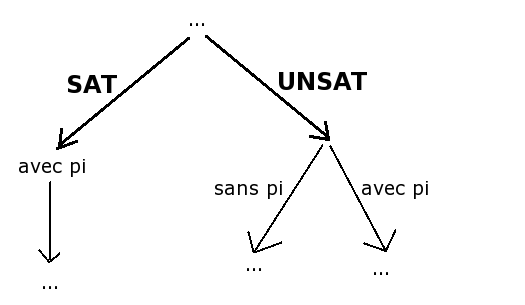
\includegraphics[scale=0.7]{./pictures/alg3.png}
    % alg3.png: 525x305 pixel, 96dpi, 13.89x8.07 cm, bb=0 0 394 229
  \end{center}
  
  La complexité de cet algorithme est beaucoup moins prévisible que celle des deux précédents, pour une même liste de prédicats, on peut avoir une complexité différente (du simple au double) selon l'ordre des éléments.
  
  Imaginons par exemple une liste où un seul élément est superflu. Dans le cas de gauche, nous analysons ce prédicat en premier, dans le cas de droite, nous l'analysons en dernier. Les points verts sur la figure signifient que le solveur a retourné \SAT après qu'on ait retiré le prédicat en question (et donc on le laisse).
  
  \begin{center}
    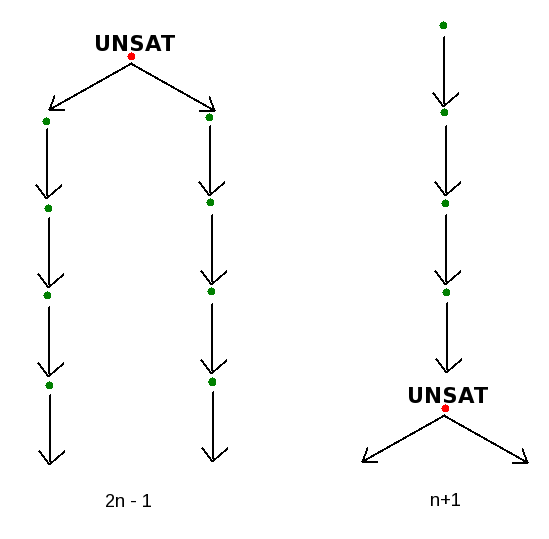
\includegraphics[scale=0.7]{./pictures/alg3_complexity.png}
    % alg3_complexity.png: 549x539 pixel, 96dpi, 14.52x14.26 cm, bb=0 0 412 404
  \end{center}

  Ici l'unité de complexité et le nombre d'appels au solveur SMT. Si $n$ est la taille de la liste de prédicats, la complexité est de $2n-1$ dans le premier cas et de $n+1$ dans le deuxième, et cela pour une même liste !
  
  La liste de prédicats qui donne le pire cas possible est celle dont tous les éléments sont insatisfiables à eux tous seuls, la complexité avoisine dans ce cas $2^{n-1}$.
  
  \bigbreak
  
  Nous allons maintenant exécuter l'algorithme sur un exemple précis. Nous avons :
  
  \begin{itemize}
    \item $p_1 \coloneqq (x = y)$
    \item $p_2 \coloneqq (x > 1)$
    \item $p_3 \coloneqq (x > 2)$
    \item $p_4 \coloneqq (y = 0)$
  \end{itemize}

  La liste $\{p_1, p_2, p_3, p_4\}$ est effectivement \UNSAT.
  
  Inutitivement, on voit que $\{p_1, p_2, p_4\}$ et $\{p_1, p_3, p_4\}$ sont les plus petits démonitateurs insatisfiables de cette liste, ce sont donc les deux résultats auxquels nous souhaitons arriver. Appliquons maintenant l'algorithme :
  
  \begin{algorithm}[H]
    $\{\strike{p_1}, p_2, p_3, p_4\}$ : \SAT\\
    $\{p_1, \strike{p_2}, p_3, p_4\}$ : \UNSAT\\
    \textbf{Fork !}\\
    \uline{Branche 1 ($\strike{p_2}$) :}\\
    \qquad $\{p_1, \strike{p_2}, \strike{p_3}, p_4\}$ : \SAT\\
    \qquad $\{p_1, \strike{p_2}, p_3, \strike{p_4}\}$ : \SAT\\
    \qquad $\mathbb{\Rightarrow}$ \textbf{Résultat :} $\{p_1, \strike{p_2}, p_3, p_4\}$\\
    \uline{Branche 2 ($p_2$) :}\\
    \qquad $\{p_1, p_2, \strike{p_3}, p_4\}$ : \UNSAT\\
    \qquad \textbf{Fork !}\\
    \qquad \uline{Branche 2.1 ($\strike{p_3}$) :}\\
    \qquad \qquad $\{p_1, p_2, \strike{p_3}, \strike{p_4}\}$ : \SAT\\
    \qquad \qquad $\mathbb{\Rightarrow}$ \textbf{Résultat :} $\{p_1, p_2, \strike{p_3}, p_4\}$\\
    \qquad \uline{Branche 2.2 ($p_3$) :}\\
    \qquad \qquad $\{p_1, p_2, p_3, \strike{p_4}\}$ : \SAT\\
    \qquad \qquad $\mathbb{\Rightarrow}$ \textbf{Résultat :} $\{p_1, p_2, p_3, p_4\}$\\
  \end{algorithm}
  
  Nous avons donc maintenant trois listes de prédicats insatisfiables, qui sont des sous-listes de la liste de départ :
  
  \begin{itemize}
    \item $\{p_1, p_3, p_4\}$
    \item $\{p_1, p_2, p_4\}$
    \item $\{p_1, p_2, p_3, p_4\}$
  \end{itemize}
  
  Cet algorithme renvoie la liste \textbf{exhaustive} des conjonctions de prédicats insatisfiables, c'est d'ailleurs pourquoi on retrouvera toujours la liste de départ. Pour l'instant, nous avons le même résultat que celui de l'algorithme naïf (mais avec une meilleure complexité).
  
  Il faut maintenant ``épurer'' cette liste pour ne conserver que les listes de prédicats \textit{minimales}, c'est-à-dire celles qui sont telles que si on supprime un élément quelconque de la liste, elle perdra toujours son insatisfiabilité (tous ses éléments lui sont nécessaires).
  
  Une fois ce test fait sur les listes trouvées, nous nous apercevons que la dernière liste ($\{p_1, p_2, p_3, p_4\}$) n'est pas minimale, elle est donc enlevée. L'algorithme retourne finalement :
  
  \begin{itemize}
    \item $\{p_1, p_3, p_4\}$
    \item $\{p_1, p_2, p_4\}$
  \end{itemize}
  
  qui sont bien les deux sous-listes minimales de $\{p_1, p_2, p_3, p_4\}$.
  
  Ce test de minimalité des conjonctions de prédicats a été en implémenté avec une approche moins naïve que celle-ci, en utilisant des masques de bits pour accélérer cette partie de l'algorithme. S'agissant là d'un détail technique sans grand rapport au reste de l'analyse, je ne le développerai pas ici.

  \newpage{}
  \section{Traduction en contraintes ILP}
  Une fois les chemins infaisables trouvés, il faut générer des contraintes ILP sur le CFG utilisables par OTAWA pour affiner (du moins on l'espère) l'estimation du WCET.

  \subsection{Cas avec deux if en séquence}
   Commençons avec un exemple simple de deux \texttt{if... then... else ...} en séquence (figure~\ref{if_2seq}). La première condition est notée \texttt{x} et la deuxième \texttt{y}, nous avons étiquettés les 4 arcs correspondants aux branchements conditionnels : \texttt{x}, \texttt{\textlnot x}, \texttt{y}, \texttt{\textlnot y}.


%   \begin{figure}
%     \centering
%     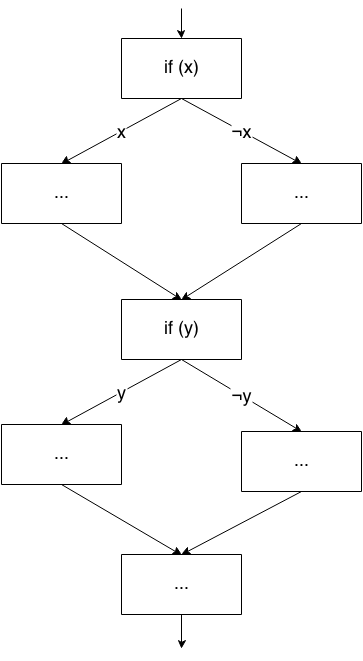
\includegraphics[scale=0.45]{./pictures/if_2seq.png}
%     % if_2seq.png: 363x661 pixel, 72dpi, 12.80x23.32 cm, bb=0 0 363 661
%     \caption{Premier exemple : deux if en séquence}
%     \label{if_2seq}
%   \end{figure}
  \begin{wrapfigure}{R}{0in}
    \centering
    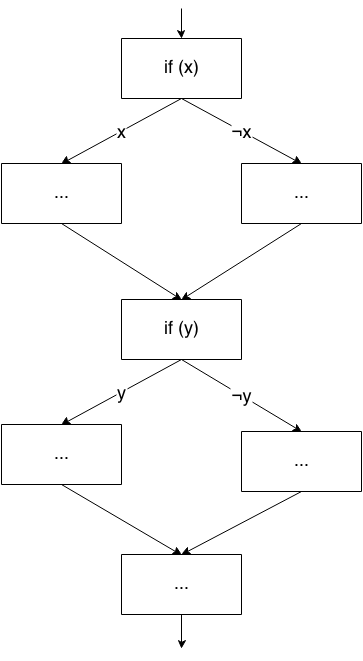
\includegraphics[scale=0.4]{./pictures/if_2seq.png}
    % if_2seq.png: 363x661 pixel, 72dpi, 12.80x23.32 cm, bb=0 0 363 661
    \caption{Premier exemple : deux if en séquence}
    \label{if_2seq}
  \end{wrapfigure}

  Nous notons $n_x$, $n_{\neg x}$, $n_y$ et $n_{\neg y}$ les variables qui représentent le nombre de fois que sont exécutés les arcs respectifs \texttt{x}, \texttt{\textlnot x}, \texttt{y}, et \texttt{\textlnot y}.

  Le problème est le suivant : nous savons que le chemin \texttt{x-y} (je note ainsi le seul chemin qui passe par les arcs notés \texttt{x} et \texttt{y}) est infaisable. Quelles contraintes ILP peut-on en déduire ?

  Attention, nous ne cherchons pas à trouver une équivalence (chemin infaisable $\Leftrightarrow$ contraintes ILP) mais simplement une implication (chemin infaisable $\Rightarrow$ contraintes ILP). Nous verrons plus loin que la perte d'information lors du passage aux contraintes ILP est irrémédiable et qu'il est parfois impossible d'avoir une équivalence.

  \medbreak

  Pour un tel chemin infaisable \texttt{x-y}, l'\textit{unique} contrainte ILP que nous générons est la suivante :

  \[ n_x \leq n_{\neg y} \]

  Intuitivement, cette contrainte est valide (c'est-à-dire qu'elle est toujours vraie si \texttt{x-y} est un chemin infaisable) :

  En effet, si \texttt{x-y} est un chemin infaisable, alors tous les chemins qui passent par \texttt{x} passeront forcément par \texttt{\textlnot y}. Donc le nombre de fois que l'arc \texttt{\textlnot y} est exécuté, noté $n_{\neg y}$, est nécessairement \textit{supérieur ou égal} au nombre de fois que l'arc \texttt{x} est exécuté, c'est-à-dire $n_x$ (c'est supérieur s'il existe des chemins \texttt{\textlnot x-y}). Cela se traduit bien par

  \[ n_x \leq n_{\neg y} \]

  On pourrait observer que de même, puisque \texttt{x-y} est un chemin infaisable, alors tous les chemins qui passent par \texttt{y} passeront forcément par \texttt{\textlnot x}, et donc que :

  \[ n_y \leq n_{\neg x} \]

  Nous allons maintenant montrer que $n_x \leq n_{\neg y} \Leftrightarrow n_y \leq n_{\neg x}$ et que par conséquent générer ces deux contraintes au lieu d'une seule est \textit{superflu}. Pour cela nous allons utiliser la propriété de flots de graphes qui dit que

  \[ n_x + n_{\neg x} = n_y + n_{\neg y} = N\]

  où N est une constante (qui représente le nombre total d'exécutions du programme). Nous avons ainsi :

  \begin{align*}
    n_x &\leq n_{\neg y} \\
    \Leftrightarrow n_x + (n_{\neg x} - n_{\neg x}) &\leq n_{\neg y} + (n_y - n_y) \\
    \Leftrightarrow (n_x + n_{\neg x}) - n_{\neg x} &\leq (n_{\neg y} + n_y) - n_y \\
    \Leftrightarrow N - n_{\neg x} &\leq N - n_y \\
    \Leftrightarrow - n_{\neg x} &\leq - n_y \\
    \Leftrightarrow n_y &\leq n_{\neg x} & \pushright{\blacksquare}
  \end{align*}

  \subsection{Cas avec trois if en séquence}
  \begin{wrapfigure}{R}{0in}
    \centering
    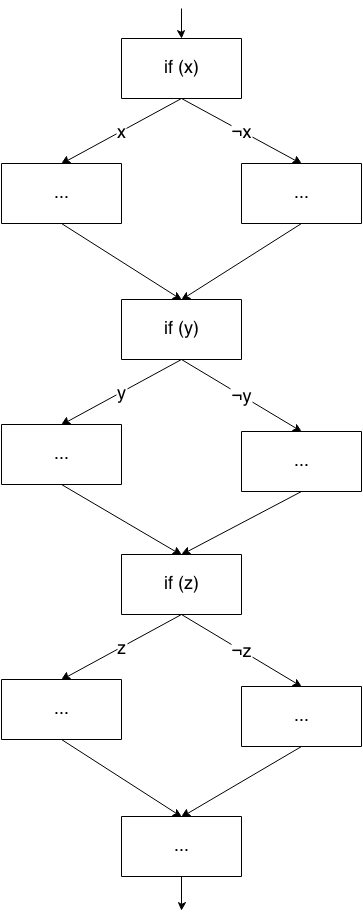
\includegraphics[scale=0.4]{./pictures/if_3seq.png}
    % if_3seq.png: 363x923 pixel, 72dpi, 12.80x32.56 cm, bb=0 0 363 923
    \caption{Deuxième exemple : trois if en séquence}
    \label{if_3seq}
  \end{wrapfigure}

  Voyons maintenant ce qui se passe lorsque l'on rajoute un autre \texttt{if... then... else ...} en séquence, ainsi que deux arcs notés \texttt{z} et \texttt{\textlnot z}.

  Supposons que \texttt{x-y-z} soit un chemin infaisable. Inutitivement, on en déduit que si un chemin passe par \texttt{x}, alors il passera par \texttt{\textlnot y} ou par \texttt{\textlnot z}. C'est-à-dire, exprimé en termes de nombre d'exécution des arcs :

  \[n_x \leq n_{\neg y} + n_{\neg z} \]

  De manière similaire, on trouve aussi que ``\texttt{x-y-z} chemin infaisable'' entraîne :

  \begin{align*}
    n_y &\leq n_{\neg x} + n_{\neg z} \\
    n_z &\leq n_{\neg x} + n_{\neg y}
  \end{align*}

  Une fois de plus, nous allons prouver que ces trois assertions sont équivalentes. Nous avons toujours la propriété de flots de graphes (cette sorte de loi des noeuds) qui dit que :

  \[ n_x + n_{\neg x} = n_y + n_{\neg y} = n_z + n_{\neg z} = N\]

  Montrons alors ces équivalences :

  \begin{align*}
    &\boxed{n_x \leq n_{\neg y} + n_{\neg z}} \\
    \Leftrightarrow& n_x \leq n_{\neg y} + (n_y - n_y) + n_{\neg z} \\
    \Leftrightarrow& n_x \leq (n_{\neg y} + n_y) - n_y + n_{\neg z} \\
    \Leftrightarrow& n_x \leq N - n_y + n_{\neg z} \\
    \Leftrightarrow& n_x + n_y \leq N + n_{\neg z} \\
    \Leftrightarrow& n_y \leq N - n_x + n_{\neg z} \\
    \Leftrightarrow& n_y \leq (n_x + n_{\neg x}) - n_x + n_{\neg z} \\
    \Leftrightarrow& \boxed{n_y \leq n_{\neg x} + n_{\neg z}} \\
    \Leftrightarrow& n_y \leq n_{\neg x} + n_{\neg z} \\
    \Leftrightarrow& n_y \leq n_{\neg x} + (N - n_z) \\
    \Leftrightarrow& n_z \leq n_{\neg x} + N - n_y \\
    \Leftrightarrow& \boxed{n_z \leq n_{\neg x} + n_{\neg y}} & \pushright{\blacksquare}
  \end{align*}

  Générer une seule de ces trois contraintes est donc suffisant. On peut remarquer que cela entraîne également la propriété suivante :

  \[
    \left.
    \begin{array}{c}
      n_x \leq n_{\neg y} + n_{\neg z}\\
      n_y \leq n_{\neg x} + n_{\neg z}\\
      n_z \leq n_{\neg x} + n_{\neg y}
    \end{array}
    \right\} \Longrightarrow n_x+n_y+n_z \leq 2(n_{\neg x} + n_{\neg y} + n_{\neg z})
  \]


  Nous voyons apparaître un motif qui se répète, que nous allons tenter de généraliser dans la prochaine section.

  \subsection{Généralisation}
  \begin{theorem}
    Pour un CFG composé de $k$ \texttt{if... then... else... } en séquence, où les arcs pris (\texttt{then}) de chacune de ses conditions sont notés $x_1$, $x_2$, ..., $x_k$ et les arcs non pris (\texttt{else}) sont notés $\neg x_1$, $\neg x_2$, ..., $\neg x_k$, on note le nombre de fois qu'un arc $x_i$ (resp. $\neg x_i$) est emprunté $n_{x_i}$ (resp. $n_{\neg x_i}$).

    Si $x_1$\texttt{-}$x_2$\texttt{-...-}$x_k$ est un chemin infaisable, alors on en déduit les $k$ contraintes ILP suivantes :

    \[\forall i \in \llbracket 1, k \rrbracket,\; n_{x_i} \leq \sum_{j \in \llbracket 1, k \rrbracket \setminus \{i\}} n_{\neg x_j} \]

    et chacune de ces contraintes est équivalente. De plus, il est immédiat que : % pourquoi on est passé en math-mode ???

    \[ \sum_{i \in \llbracket 1, k \rrbracket} n_{x_i} \leq (k-1) \sum_{i \in \llbracket 1, k \rrbracket} n_{\neg x_i} \]
  \end{theorem}

  On pourra remarquer que les CFG contenant des conditions du type \texttt{if... then...} sans \texttt{else...} ne diffèrent pas du cas étudié (avec \texttt{else}) puisqu'il y a toujours deux arcs sortant du bloc de base qui calcule la condition, la différence étant que l'arc non pris pointe sur le bloc de fin de condition au lieu de pointer sur un bloc qui lui-même pointera vers ce bloc de fin de condition.


  \subsection{Limitations des contraintes ILP}
  \begin{wrapfigure}{r}{0in}
    \centering
    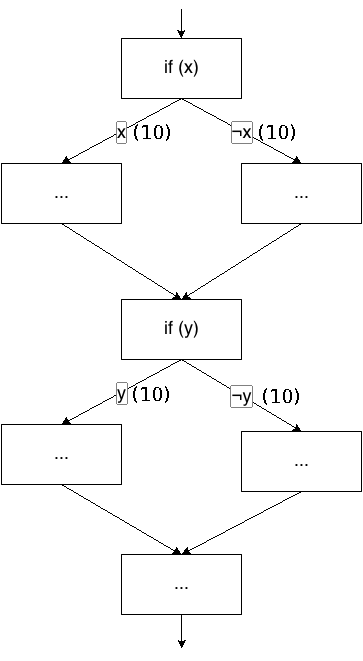
\includegraphics[scale=0.4]{./pictures/ambiguite_ilp.png}
    % ambiguite_ilp.png: 363x661 pixel, 72dpi, 12.80x23.32 cm, bb=0 0 363 661
    \caption{Exemple du manque d'expressivité des contraintes ILP}
    \label{ambiguite ilp}
  \end{wrapfigure}

  Les contraintes ILP manquent toutefois d'expressivité pour représenter toute l'information contenue dans la notion de ``chemin infaisable'', comme expliqué dans un article du WCET 2005 workshop :

  \begin{quote}
    ``This is because the usual ILP formulation introduces formal variables for the execution counts of the nodes and edges in the Control Flow Graph (CFG) of the program. Since the variables denote aggregate execution counts of basic blocks, it is not possible to express certain infeasible path patterns as constraints on these variables.''~\cite{wcet05}
  \end{quote}

  En effet, si on considère l'exemple de la figure~\ref{ambiguite ilp}, où les valeurs entre paranthèses sur chaque arc représentent le nombre de fois que l'arc est exécuté dans le scénario considéré, il est impossible de déterminer si l'on a un chemin infaisable (en tout cas un chemin qui n'est jamais pris) ou non à partir des seules variables $n_x$, $n_{\neg x}$, $n_y$, $n_{\neg y}$ !

  Il se pourrait, par exemple, que les 20 exécutions du CFG consistent en 10 fois le chemin \texttt{x-\textlnot y} et 10 fois le chemin \texttt{\textlnot x-y}. Dans ce cas, le chemin \texttt{x-y} n'est effectivement jamais pris.

  Mais il se pourrait aussi, que l'on ait 10 exécutions qui passent par le chemin \texttt{x-y} !

  Dans ces conditions, on ne peut pas signifier à OTAWA si ce scénario (avec ces comptes d'exécution) est viable ou non, et il sera donc inclus dans le calcul du WCET. Les contraintes ILP ne permettent pas d'exprimer tout ce que l'on sait à partir de l'hypothèse ``chemin infaisable''.

  Il faut prendre conscience de cette limitation à l'étape ``utilisation des chemins infaisables trouvés'', de cette perte d'information, mais cela ne signifie pas nécessairement que le choix de la génération de contraintes ILP est mauvais. L'autre alternative serait de faire de la réécriture de graphe pour faire apparaître (ou plutôt disparaître en l'occurence) les chemins infaisables sur le CFG, mais c'est bien plus coûteux, et aussi plus compliqué.

  \'Etant donné qu'un membre de l'équipe TRACES travaille justement sur la réécriture de CFG, une collaboration sur ce sujet est envisageable pour ma thèse.

  \newpage{}
  \addcontentsline{toc}{section}{Conclusion}
  \section*{Conclusion}
  En me basant sur l'outil open-source OTAWA~\cite{otawa} développé par l'équipe TRACES, j'ai développé une analyse des chemins infaisables de programmes écrits en langage assembleur, dans le but ultime d'améliorer notre estimation du pire temps d'exécution. OTAWA m'a fourni les outils nécessaires pour m'abstraire des spécificités de chaque langage machine et me permettre de travailler sur un langage générique, ainsi que de nombreuses facilités pour parcourir le flot d'un programme en considérant ce dernier comme un graphe (CFG).
  
  En utilisant l'interprétation abstraite~\cite{cousot} comme base théorique, j'ai représenté les états de l'exécution d'un programme assemmbleur par des listes de prédicats qui décrivent l'état du système (registres et mémoire). J'a utilisé une technique énumération implicite des chemins (IPET) du CFG, et tout en parcourant le chemin et en faisant évoluer la liste de prédicats, j'ai cherché des inconsistances dans cette liste, afin d'identifier des chemins infaisables.
  
  J'ai utilisé un solveur SMT reconnu, CVC4~\cite{smt_cvc4}, pour détecter des insatisfiabilités dans ces prédicats. Une fois l'insatisfiabilité levée (et donc un chemin infaisable détecté), il a fallu en extraire les chemins infaisables minimaux pour en maximiser l'exploitabilité.
  
  Une fois l'exécution du programme finie, ces prédicats ont été traduits en contraintes ILP pour être ensuite injectées dans le calcul de WCET d'OTAWA et l'améliorer.
  
  Bien que le programme d'analyse soit fonctionnel et trouve effectivement les chemins infaisables sur les benchmarks simples sur lesquels nous l'avons testé, il subit encore certaines limitations, dont la plus importante est probablement l'absence de gestion des boucles.
  
  L'extension de cette analyse (notamment à des programmes avec boucles) fera l'objet d'une thèse au sein de la même équipe l'année prochaine, et peut-être de collaborations avec d'autres membres de l'équipe, en particulier en ce qui concerne l'exploitation des chemins infaisables trouvés.

\newpage{}
%\bibliographystyle{plain}
\addcontentsline{toc}{section}{Références}
\begin{thebibliography}{1}
    
    \bibitem{cousot}Patrick Cousot and Rahida Cousot. 1992. \textit{Abstract interpretation and application to logic programs}. J. Log. Program. 13, 2-3 (July 1992), 103-179. http://dx.doi.org/10.1016/0743-1066(92)90030-7
    \bibitem{nielson}Flemming Nielson, Hanne R. Nielson, and Chris Hankin. 1999. \textit{Principles of Program Analysis}. Springer-Verlag New York, Inc., Secaucus, NJ, USA.
    \bibitem{entcs}\textit{Electronic Notes in Theoretical Computer Science (Entcs)}. Elsevier Sci. Pub. B. V., Amsterdam, The Netherlands, The Netherlands. http://dx.doi.org/10.1016/j.entcs.2010.09.014
    \bibitem{wcet05} T. Chen, T. Mitra, A. Roychoudhury, and V. Suhendra. \textit{Exploiting branch constraints without exhaustive path enumeration}. In Int’l Workshop on WCET Analysis, 2005.
    \url{http://www.comp.nus.edu.sg/~tulika/wcet05.pdf}
    \bibitem{intlconf11}S. Andalam, P. Roop, and A. Girault. \textit{Pruning Infeasible Paths for Tight WCRT Analysis of Synchronous Programs}. In Intl’ Conf. on Design, Automation and Test in Europe (DATE), 2011.
    \bibitem{smtintro}Leonardo De Moura and Nikolaj Bjørner. 2011. \textit{Satisfiability modulo theories: introduction and applications}. Commun. ACM 54, 9 (September 2011), 69-77.
    \url{http://doi.acm.org/10.1145/1995376.1995394}
    \bibitem{otawa}Hugues Cassé, Florian Birée, Pascal Sainrat. Multi-architecture Value Analysis for Machine Code (regular paper). Dans / In : Workshop on Worst-Case Execution Time Analysis, Paris, 09/07/2013, (Eds.), OASICs, Dagstuhl Publishing, p. 42-52, juillet / july 2013.

    \bibitem{ARM instruction set} ARM Instruction Set Quick Reference Card. \url{http://infocenter.arm.com/help/topic/com.arm.doc.qrc0001l/QRC0001_UAL.pdf}
    \bibitem{SMT-COMP} SMT-COMP: Satisfiability Modulo Theories Competition. Édition 2012. \url{http://smtcomp.sourceforge.net/2012/}

    \bibitem{smt_z3} SMT solver Z3. \url{http://z3.codeplex.com/}
    \bibitem{smt_cvc4} SMT solver CVC4. \url{http://cvc4.cs.nyu.edu/web/}
    \bibitem{smt_mathsat5} SMT solver MathSAT 5. \url{http://mathsat.fbk.eu/documentation.html}
    \bibitem{smt_boolector} SMT solver Boolector. \url{http://fmv.jku.at/boolector/}
    \bibitem{smt_sonolar} SMT solver SONOLAR. \url{http://www.informatik.uni-bremen.de/~florian/sonolar/}
    \bibitem{smt_mistral} SMT solver MISTRAL. \url{http://www.cs.wm.edu/~tdillig/mistral/index.html}
    \bibitem{smt_verit} SMT solver VeriT. \url{http://www.verit-solver.org/veriT-download.php}
    \bibitem{smt_barcelogic} SMT solver Barcelogic. \url{http://www.lsi.upc.edu/~oliveras/bclt-main.html}
\end{thebibliography}
\end{document}
